\pagestyle{empty} % Limpa o cabeçalho e o rodapé
\onehalfspacing % Espaçamento entre-linhas de 1,5
% \hyphenpenalty=10000 % To prevent hyphenation
\pretolerance=10000 % To avoif overful lines
%\selectlanguage{english}
\selectlanguage{brazilian}
\setcounter{ex}{0} % counter for exercises
%\pagenumbering{arabic} % Uncomment this line if you want renumber pages for each chapter
\renewcommand{\chaptername}{Tutorial}
\chapter{Homologia Dinâmica: Buscas em POY, sensibilidade, comprimentos de ramos e alinhamentos implícitos}\label{tut10}
\rhead{\tiny Instituto de Biociências --USP: BIZ0433 - Inferência Filogenética: Filosofia, Método e Aplicações}
\cfoot{\tiny \cc \ccby \ccsa \href{http://creativecommons.org/licenses/by-sa/4.0/}{Creative Commons Attribution-ShareAlike 4.0 International License}}
%\vspace{5pt}
{\large \sc BIZ0433 - Inferência Filogenética: Filosofia, Método e Aplicações.}\par
%\vspace{10pt}
\par
\minitoc % for table of contents within the chapter
\newpage
\section*{}\addcontentsline{toc}{section}{Objetivo}
\onehalfspacing
\vspace*{5pt}
\begin{center}
\emph{\begin{large}Objetivo\end{large}}\label{tut10:Objetivo}
\vspace{2pt}
\end{center}
%% TEXTO DO RESUMO
O objetivo deste tutorial é apresentar novos conceitos associados a análise de sequências nucleotídicas, principalmente utilizando otimização direta de dados moleculares. O tutorial está centrado no conceito de análise de sensibilidade para o qual será apresentado algumas ponderações epistemológicas -- estas devem ser suplementadas pela literatura citada no tutorial --, bem como a implementação destas análises em POY. Antes disso, você irá conhecer como POY implementa novas tecnologias de busca em análises com tempo determinado, uma ferramenta muito útil deste programa. O tutorial também explora o uso de FigTree e Inkscape na preparação de figuras que contém diagramas de sensibilidade. Por fim, o tutorial mostra como o POY apresenta topologias com seus respectivos comprimentos de ramo e o alinhamento implícito relacionado com análises de homologia dinâmica. Os arquivos associados a este tutorial estão disponíveis no \href{https://github.com/fplmarques/cladistica/tree/main/tutorials/}{GitHub}. Você baixar todos os tutoriais com o seguinte comando:

\begin{center}
\small \texttt{svn checkout https://github.com/fplmarques/cladistica/trunk/tutorials/}\\
\end{center}


\newpage
\pagestyle{fancy} % Inclui o cabeçalho definido no meta.tex
%\pagenumbering{arabic} % Números das páginas em arábicos
\begin{refsection}
\renewcommand*{\finalnamedelim}{\addspace\&\space} % Usar '&' ao invés de 'e'.
%
%% color base pairs
\newcommand{\A}{\textcolor{green}{\textbf{A}}}
\newcommand{\C}{\textcolor{blue}{\textbf{C}}}
\newcommand{\G}{\textcolor{gray}{\textbf{G}}}
\newcommand{\T}{\textcolor{red}{\textbf{T}}}
\newcommand{\gap}{\textcolor{black}{\textbf{-}}}


%%%%%%%%%%%%%%%%%%%%%%%%%%%% HERE TEXT STARTS %%%%%%%%%%%%%%%%%%%%%%%%%%%%
\section{Novas tecnologias de busca em POY}\label{tut10:search}\\

No tutorial anterior utilizamos os algoritmos mais simples de busca existentes em POY (\textit{i.e.}, RAS+SWAP). No entanto, o POY também permite que a maioria dos algoritmos implementados em TNT \parencite{GoloboffEtAl_2008}, considerados novas tecnologias de busca \parencite{Goloboff_1999,Nixon_1999}, sejam implementados em buscas de homologia dinâmica. No entanto, devido às propriedades dos algoritmos de POY, algumas implementações requerem uma série de transformações dos dados que podem ser complexas para o usuário com pouca experiência. Considere por exemplo a implementação de \textit{ratchet} \parencite{Nixon_1999}. Esse algoritmo atribui pesagem diferencial à uma proporção de seus caracteres, executa busca e refinamento na matriz, retorna ao esquema de pesagem inicial e avalia o custo da(s) topologia(s) em comparação àquela(s) inicialmente retida(s) na memória do programa. Em homologia dinâmica, é necessário transformar os caracteres dinâmicos em caracteres estáticos temporariamente para a implementação de \textit{ratchet}. Isso é necessário porque a noção de caráter em otimização direta varia a cada ciclo de otimização durante as buscas. Portanto, a implementação em POY de algoritmos de dependem de homologia estática, como é o caso de \textit{ratchet}, requer uma série de instruções no \textit{script} que, como verão, são de certa forma desnecessárias na maioria das análises que você irá fazer.

Para facilitar o uso de POY, o desenvolvedores do programa criaram o comando ``\texttt{search}'' que implementa todas essas novas tecnologias de busca sem que o usuário tenha que se preocupar com as linhas de comando de cada uma das estratégias de refinamento. Por \textit{default}, o comando ``\texttt{search}'' inclui a construção inicial de uma árvore de Wagner, em seguida, implementa \textit{branch swapping} via TBR (veja Tutorial \ref{tut4}, Seção \ref{tut4:search}), \textit{ratchet} \parencite{Nixon_1999} e \textit{tree fusing} \parencite{Goloboff_1999}, sequencialmente. Esse ciclo de algoritmos é considerado pelo POY como repetições independentes, cujo número de iterações dependerá da complexidade de seus dados e dos argumentos implementados no comando ``\texttt{search}''.

Os argumentos do comando ``\texttt{search}'' permitem uma série de controles (veja item 3.3.22, página 119, do manual do programa). Por \textit{default} o comando faz a busca por uma hora e usa 2 Gb de memória RAM em seu computador. Esse comando seria expresso literalmente da seguinte forma: \texttt{search(max\_time:0:1:0,min\_time:0:1:0,memory:gb:2)}\footnote{ No entanto, como estes são os argumentos originais do comando, bastaria escrever ``\texttt{search()}''.}. Nesta linha de comando, o argumento ``\texttt{max\_time:0:1:0}'' define o máximo de tempo estipulado para análise em dias:horas:minutos, o argumento ``\texttt{min\_time:0:1:0}'' define o mínimo de tempo estipulado para análise da mesma forma, e ``\texttt{memory:gb:2}'' controla o máximo de memória alocada durante a execução. Este último restringe o número de topologias retidas na memória durante as buscas. O número de repetições independentes, neste caso, dependerá apenas da complexidade de seus dados, ou seja, o tempo necessário para completar uma iteração. Há uma série de outros argumentos para este comando e o leitor deve consultar o manual do programa caso esteja interessado em implementar alguns deles em suas análises. No exemplo abaixo iremos explorar apenas um deles (\textit{i.e.}, \texttt{max\_time:d:m:s}), pois é o mais utilizado.

	Considere o \textit{script} abaixo:


\begin{lstlisting}[caption= conteúdo do arquivo script1.poy (Tutorial \ref{tut10}),label=tut10:search:script1]
read("partition2.fas")
set(root:"Taxon1")
search(max_time:0:0:0.1)
select()
report(trees)
report(searchstats) 
exit()
\end{lstlisting}

Neste \textit{script} o arquivo \texttt{partition2.fas} é lido pelo POY [linha 1], o táxon \texttt{Taxon1} é utilizado como raiz [2] e a busca será feita por 1/10 minutos [3] após a qual as topologias únicas e mais curtas serão retidas [4] e impressas [5] juntamente com a estatística da busca [6].

Execute este \textit{script} da seguinte maneira:\\

\shellcmd{poy5.1.2a script1.poy >std.out 2>std.err \&}\\

Nesta linha de comando, o \textit{prompt} do terminal será liberado logo após você executá-lo, pois o caráter ``\texttt{\&}'' no final da linha faz com que o programa seja executado no \textit{background}. Para saber se o programa terminou a execução pressione a tecla \texttt{ENTER} após alguns segundos. Em algum momento você deverá obter:\\

\scriptsize

alan@turing:~/Desktop/tutorials/tutorial\_10\$ poy5.1.2a script1.poy >std.out 2>std.err \&

[1] 3992\footnote{ número do processo, ou seja, o número que a máquina atribuiu para a linha de comando que você acaba de executar.}
\vspace{20pt}
alan@turing:~/Desktop/tutorials/tutorial\_10\$ 

[1]+  Concluído              poy5.1.2a script1.poy >std.out 2> std.err\\

\normalsize

Observe os redirecionamentos implementados na linha de comando (veja Tutorial \ref{tut1})\footnote{ mais informações sobre \textit{standard I/O streams} em linux veja \url{http://linux.about.com/library/cmd/blcmdl3\_stderr.htm}}. O primeiro deles (\textit{i.e.}, ``\texttt{>std.out}''), os registros de saída convencionais de POY -- geralmente aqueles que direcionamos para arquivos, como por exemplo \texttt{report(``trees.tre'',trees)} --, ou os chamados \textit{stdout}, são direcionados para o arquivo \texttt{std.out}. O segundo deles (\textit{i.e.}, ``\texttt{>std.err}''), os registros de execução ou erro convencionais de POY -- geralmente aqueles impressos no terminal durante a execução --, ou os chamados \textit{stderr}, são direcionados para o arquivo \texttt{std.err}. Vamos examinar o conteúdos destes dois arquivos.

Se você examinar o conteúdo do arquivo \texttt{std.out}, você deverá encontrar algo semelhante ao que está impresso abaixo:


\scriptsize

(Taxon1,((Taxon5,(Taxon2,(Taxon4,Taxon9))),((Taxon3,Taxon8),(Taxon6,(Taxon10,Taxon7)))));

(Taxon1,((Taxon5,(Taxon2,(Taxon4,Taxon9))),(Taxon6,(Taxon8,(Taxon3,(Taxon10,Taxon7))))));

Search~Stats:

\#~of~Builds~+~TBR~~16

\#~of~Fuse~~~~~~~~~~93

\#~of~Ratchets~~~~~~11

Tree~length~~~~~~~~Number~of~hits

191.~~~~~~~~~~~~~~~195

192.~~~~~~~~~~~~~~~7

193.~~~~~~~~~~~~~~~2

194.~~~~~~~~~~~~~~~5

195.~~~~~~~~~~~~~~~3

196.~~~~~~~~~~~~~~~2

197.~~~~~~~~~~~~~~~1

198.~~~~~~~~~~~~~~~1

199.~~~~~~~~~~~~~~~1

\normalsize

Neste arquivo de saída, as duas primeiras linhas contém as duas topologias encontradas na análise, impressas nesse arquivo pelo comando ``\texttt{report(trees)}'' e as demais linhas registram as estatísticas de busca, impressas nesse arquivo pelo comando ``\texttt{report(searchstats)}'' do \textit{script} \ref{tut10:search:script1}. Os registros de busca indicam que durante o tempo estipulado (1/10 minutos) POY realizou 16 réplicas independentes, 11 iterações de \textit{ratchet} e 93 iterações de \textit{tree fusing} sendo que em 195 ocasiões obteve uma topologia com 191 transformações. Lembre-se que eu poderia direcionar esses arquivos de saída para arquivos individuais implementando a seguinte linha de comando: \texttt{report(''treefile.tre'', trees,''searchstatistics.txt'', searchstats)}.

Examine o arquivo \texttt{>std.err}. Este registra toda a execução de POY que você acabou de implementar. Ele deverá conter registros semelhantes aos impressos abaixo, onde cada etapa da busca é marcada por ''\texttt{<-- ...}'':

\scriptsize

...

Information~:~The~file~partition2.fas~contains~sequences~of~10~taxa,~each

~~~~~~~~~~~~~~sequence~holding~1~fragment.~\textcolor{red}{<--~Leitura~do~arquivo~de~entrada}

Status~:~RAS~+~TBR~:~0~

Status~:~RAS~+~TBR~:~0~Searching~on~tree~number~1

Status~:~Wagner~:~2~of~10~--~Wagner~tree~with~cost~36.~\textcolor{red}{<--~Construção~da~árvore~de~Wagner}

...

Status~:~Wagner~:~9~of~10~--~Wagner~tree~with~cost~172.

Status~:~Wagner~Finished

Status~:~Building~Wagner~Tree~Finished

Status~:~TBR~:~191~191.~\textcolor{red}{<--~Inicio~do~refinamento~por~TBR}

Status~:~TBR~Finished

Status~:~Automated~Search~:~0~Best~tree:~191.;~Time~left:~6~s;~Hits:~1~\textcolor{red}{<--~Melhor~topologia~depois~de~TBR}

Status~:~Transforming~:~1~of~1~--~~transformations~applied~\textcolor{red}{<--~Tranformação~dos~caracteres~em~homologia~estática}

Status~:~Transforming~:~0~of~1~--~~characters~transformed

Status~:~Transforming~Finished

Status~:~Diagnosis~:~1~of~1~--~Recalculating~trees

Status~:~Diagnosis~Finished

Status~:~Implied~Alignments~:~1~of~19~--~vertices~calculated

Status~:~Implied~Alignments~:~2~of~19~--~vertices~calculated

...

Status~:~Implied~Alignments~:~16~of~19~--~vertices~calculated

Status~:~Implied~Alignments~:~17~of~19~--~vertices~calculated

Status~:~Implied~Alignments~Finished

Status~:~Static~Approximation~Finished~\textcolor{red}{<--~Tranformação~em~homologia~estática~termina~após~ler~alinhamento~implícito}

Status~:~Loading~Characters~:~0~of~10~--~Storing~the~character~specifications

Status~:~Loading~Characters~:~1~of~10~--~Storing~the~character~specifications

...

Status~:~Loading~Characters~:~9~of~10~--~Storing~the~character~specifications

Status~:~Loading~Characters~:

~~~~~~~~~10~of~10~--~Storing~the~character~specifications

Status~:~Loading~Characters~Finished

Status~:~Transforming~:~1~of~1~--~~transformations~applied

Status~:~Transforming~:~138~of~1~--~~characters~transformed

Status~:~Transforming~Finished

Status~:~Diagnosis~:~0~Recalculating~original~tree

Status~:~Diagnosis~Finished

Status~:~Diagnosis~:~1~of~1~--~Recalculating~trees

Status~:~Diagnosis~Finished

Status~:~Perturb~Iteration~:~1~of~4~~\textcolor{red}{<--~Inicio~do~algoritimo~de~\textit{ratchet}}

Status~:~Ratcheting~:~0~of~1~--~trees~in~the~current~optimum

Status~:~Diagnosis~:~0~Recalculating~original~tree

Status~:~Diagnosis~Finished

Status~:~Ratcheting~:~1~of~1~--~trees~in~the~current~optimum

Status~:~TBR~:~234~234.

Status~:~TBR~Finished

Status~:~Diagnosis~:~0~Recalculating~original~tree

Status~:~Diagnosis~Finished

Status~:~Ratcheting~Finished

Status~:~Perturb~Iteration~:~2~of~4~--~

...

Status~:~Perturb~Iteration~:~4~of~4~--~

Status~:~Ratcheting~:~0~of~1~--~trees~in~the~current~optimum

Status~:~Diagnosis~:~0~Recalculating~original~tree

Status~:~Diagnosis~Finished

Status~:~Ratcheting~:~1~of~1~--~trees~in~the~current~optimum

Status~:~TBR~:~225~225.

Status~:~TBR~Finished

Status~:~Diagnosis~:~0~Recalculating~original~tree

Status~:~Diagnosis~Finished

Status~:~Ratcheting~Finished

Status~:~Perturb~Iteration~Finished

Status~:~Diagnosis~:~0~Recalculating~original~tree

Status~:~Diagnosis~Finished

Status~:~Ratcheting~:~1~of~1~--~trees~in~the~current~optimum

Status~:~TBR~:~225~225.

Status~:~TBR~Finished

Status~:~Diagnosis~:~0~Recalculating~original~tree

Status~:~Diagnosis~Finished

Status~:~Ratcheting~Finished

Status~:~Perturb~Iteration~Finished

Status~:~Diagnosis~:~0~Recalculating~original~tree

Status~:~Diagnosis~Finished~\textcolor{red}{<--~Termina~a~iteração~após~TBR~final}

Status~:~Automated~Search~:~0~Best~tree:~191.;~Time~left:~6~s;~Hits:~2

...

Status~:~Automated~Search~:~0~Best~tree:~191.;~Time~left:~6~s;~Hits:~1~\textcolor{red}{<--~Subsequentes~iterações}

...

Status~:~Automated~Search~:~0~Best~tree:~191.;~Time~left:~6~s;~Hits:~2

...

Status~:~Automated~Search~:~0~Best~tree:~191.;~Time~left:~3~s;~Hits:~5

...

Status~:~Automated~Search~:~0~Best~tree:~191.;~Time~left:~-0~s;~Hits:~6

Status~:~Automated~Search~Finished

Status~:~RAS~+~TBR~Finished

Status~:~Fusing~Trees~:~0~\textcolor{red}{<--~\textit{tree~fusing~no~final}}

Status~:~Fusing~Trees~Finished

Status~:~Automated~Search~Finished

Information~:~The~search~evaluated~16~independent~repetitions~with~ratchet~and~fusing~for~93~generations.~The~shortest~tree~was~found~6~times.

\normalsize

Estes arquivos de saída de POY são úteis para documentar a análise e permitir avaliar o comportamento de determinadas estratégias de busca (o que transcende os objetivos desse tutorial) e identificar problemas de execução. Desta forma, é interessante sempre redirecionar estas informações de saída em suas análises.


\section{Análise de sensibilidade}\label{tut10:sa}

\subsection{Contextualização}\label{tut10:sa:context}

Em termos gerais, análise de sensibilidade objetiva acessar a relação existente entre parâmetros analíticos e resultado \parencite{Saltelli_2000}. Dentro do contexto de análises filogenéticas de dados moleculares, \textcite{Wheeler_1995} foi o primeiro a avaliar de forma sistemática a relação entre de parâmetros de alinhamento e resultados de inferência filogenética. Em sua concepção inicial, a análise sensibilidade foi considerada uma etapa necessária que precede a análise de congruência. Esta última tem como objetivo identificar o conjunto de parâmetros analíticos que maximiza congruência de caracteres entre partições de dados \parencite[veja][]{Wheeler_1995,Wheeler_and_Hayashi_1998, Ramirez_2006}.

O uso de análise de sensibilidade em inferência filogenética é controversa. Há duas justificativas predominantes para seu uso em inferência filogenética. A primeira delas é que ela permite acessar níveis de suporte de determinados clados \parencite[\textit{e.g.},][]{Wheeler_and_Hayashi_1998,Giribet_2003}. A outra é que estas análises são úteis e necessárias para entender a relação existente entre premissas analíticas e resultados -- principalmente diante da observação de que parâmetros de alinhamento são componentes arbitrários e inevitáveis em análises filogenéticas de dados moleculares \parencite[veja][]{Giribet_and_Wheeler_2007}.

\textcite{Grant_and_Kluge_2003}, ao contrário, argumentam que o uso de análise de sensibilidade em inferência filogenética não possui base epistemológica e portanto não pode ser justificado \parencite[veja resposta em][]{Giribet_and_Wheeler_2007}. Segundo esses autores, a análise de sensibilidade não deve ser considerada um método científico, pois não permite teste de hipóteses, nem um método heurístico, pois não permite identificar hipóteses ambiguamente ou pouco corroboradas pelos dados disponíveis. Independentemente destas disputas filosóficas, vamos aprender como essas análises são feitas e a interpretação dos resultados requer reflexão sobre os pontos levantados por esses autores \parencite{Grant_and_Kluge_2003,Giribet_and_Wheeler_2007}. Minha recomendação é que consultem a literatura que discute o tema caso venham a implementar análises de sensibilidade em seus estudos.

\subsection{Implementação}\label{tut10:sa:implementation}

Há várias formas de implementar análises de sensibilidade em POY\footnote{ essas análises podem ser executadas dentro do contexto de homologia estática. Por exemplo, nada impede que os protocolos que exploramos aqui sejam implementados em TNT.} e sua implementação depende, em última instância, de quais parâmetros analíticos você quer submeter à análise de sensibilidade. Considere por exemplo a base de dados utilizada no Tutorial \ref{tut9}, Seção \ref{tut9:context:partitions}. As partições apresentadas na ocasião possuem dados que não estavam sujeitos a alinhamento (\textit{i.e.}, \texttt{partition1.fas}), dados sujeitos a alinhamento (\textit{i.e.}, \texttt{partition2.fas}) e uma matriz de dados fenotípicos (\textit{i.e.}, \texttt{partition3.tnt}). Nossa primeira análise destas partições considerou custos idênticos para todas as transformações. Desta forma, a primeira possibilidade seria avaliar como os resultados dependem desta premissa inicial simplesmente atribuindo custos diferenciais para INDELs e substituições (veja Seção \ref{tut9:context:tcm} daquele tutorial). No entanto, há varias outras possibilidades. Na realidade, infinitas! Você poderia considerar diferentes pesos para cada uma das partições, já que elas diferem de tamanho. Você poderia excluir a terceira posição da partição que inclui regiões codificantes; e por que não as primeiras e segundas também. Você poderia dar pesos diferenciais para dados genotípicos \textit{vs.} fenotípicos. Enfim, o número de parâmetros passíveis de exame são inúmeros, mesmo para essas 3 partições, e não há forma objetiva de identificar quais parâmetros serão avaliados. Esse é parte dos argumentos de \textcite{Grant_and_Kluge_2003} contra análise de sensibilidade.

Tradicionalmente, no entanto, as análises de sensibilidade centram em avaliar os custos de INDELs (algumas vezes diferenciando entre \textit{gaps} de abertura e extensão), transversões e transições \parencite{Wheeler_1995, Wheeler_and_Hayashi_1998, Giribet_and_Wheeler_1999, Phillips_et_al_2000, Giribet_2003, Wheeler_and_Giribet_2009}. Em POY isso é feito implementando matrizes de custo (\textit{i.e.}, matrizes de Sankoff) em diferentes buscas como foi feito na seção \ref{tut9:context:tcm} do Tutorial \ref{tut9}.

O conjunto de funções de custo avaliado durante a análise de sensibilidade define seu espaço de parâmetros (\textit{i.e., parameter space}). Considere por exemplo os arquivos contendo matrizes de Sankoff disponíveis no diretório \texttt{tutorial\_10}. São 9 arquivos nos quais as razões de custo entre transversões e transições podem ser de 1:1, 2:1 e 1:2; ao passo em que as razões de custo entre INDELs e substituições podem ser 1:1, 2:1 e 4:1\footnote{ observe o conteúdo destes arquivos para ver como os custos absolutos das transformações expressam as razões de custo que dão nome aos arquivos.}, respectivamente. Os nomes desses arquivos referem-se às razões de custo expressas em seu conteúdo; por exemplo, o arquivo \texttt{m421} expressa a razão de custo 4:2:1 para INDELs:transversões:transições, respectivamente. Neste caso, transições recebem custo igual a 1, transversões igual a 2 e \textit{gaps} igual a 8.

Suponha que você queira avaliar a sensibilidade dos seus resultados em relação às razões de custo entre INDELs e substituições e considere que as matrizes de custo nos arquivos \texttt{m111}, \texttt{m211} e \texttt{m411} definem meu espaço de parâmetros. O primeiro passo seria fazer três análises filogenéticas considerando uma função de custo distinta para cada uma delas. 

	Considere o \textit{script} abaixo:\\

\begin{lstlisting}[caption= Exemplo de \textit{script} para implementar análises de sensibilidade (veja \texttt{tutorial\_10/script2.poy}).,label=tut10:sa:implementation:script1]
read(prealigned:("partition1.fas", tcm:("m111")))
read("partition2.fas","partition3.tnt")
transform(names:("partition2.fas"),(tcm:("m111")))
set(root:"Taxon1")
search(max_time:0:00:1)
select()
report("trees_m111.tre",trees:(total),
"scores_m111.sts",treestats,searchstats)
exit()
\end{lstlisting}

Neste \textit{script}, a matriz de custo \texttt{m111} é implementada nos dados moleculares -- embora \texttt{partition1.fas} não esteja sujeito à alinhamento -- e os resultados são direcionados para arquivos correspondentes às matrizes de custo\footnote{ caso tenha dificuldade de compreender os demais comandos deste \textit{script} revise o Tutorial \ref{tut9} e/ou consulte a documentação do programa.}. Seguindo a lógica deste \textit{script}, a análise de sensibilidade gerará três arquivos de árvores (\textit{i.e.}, \texttt{trees\_m111.tre}, \texttt{trees\_m211.tre} e \texttt{trees\_m411.tre} -- veja diretório \texttt{tutorial\_10}). Subsequentemente, você poderia inspecionar visualmente as topologias resultantes para identificar os clados que são dependentes dos parâmetros de alinhamento. No entanto, essa tarefa pode consumir um bom tempo e há ferramentas disponíveis que podem ser úteis nessa tarefa. É o que veremos a seguir.

\subsection{Avaliação}\label{tut10:sa:evaluation}

Em dados reais, raramente você terá tempo e paciência para inspecionar visualmente os resultados de uma análise de sensibilidade. Há duas ferramentas disponíveis para este propósito. A primeira delas é o aplicativo Cladescan \parencite[][; disponível para baixar \href{https://rc.fas.harvard.edu/resources/documentation/software/cladescan/}{aqui}]{Sanders_2010}. Alternativamente, \textcite{Machado_2014} desenvolveu o YBYRÁ, um aplicativo mais versátil e rápido quando comparado ao Cladescan. Finalmente, algumas ferramentas de visualização de árvores \parencite[\textit{e.g.}, FigTree;][]{Rambaut_2006} são muito úteis para esse propósito (veja Tutorial \ref{tut2}). O resultado de uma análise de sensibilidade é ilustrado na Figura \ref{tut10:fig:sens_plot}. Essa figura foi gerada a partir da análise simultânea e individuais dos dados nos arquivos \texttt{partition1.fas}, \texttt{partition2.fas} e \texttt{partition3.tnt}. Ela mostra a frequência de cada um dos clados da análise simultânea na topologias recuperadas pelas análises individuais. 


%%%%%%%%%%%%%%%%%%%%%%%%%%% FIGURA TAP%%%%%%%%%%%%%%%%%%%%%%%%%%%
%  \vspace{-1em}
  \begin{figure}[H]
    %\ffigbox[\FBwidth]
       \centering
      {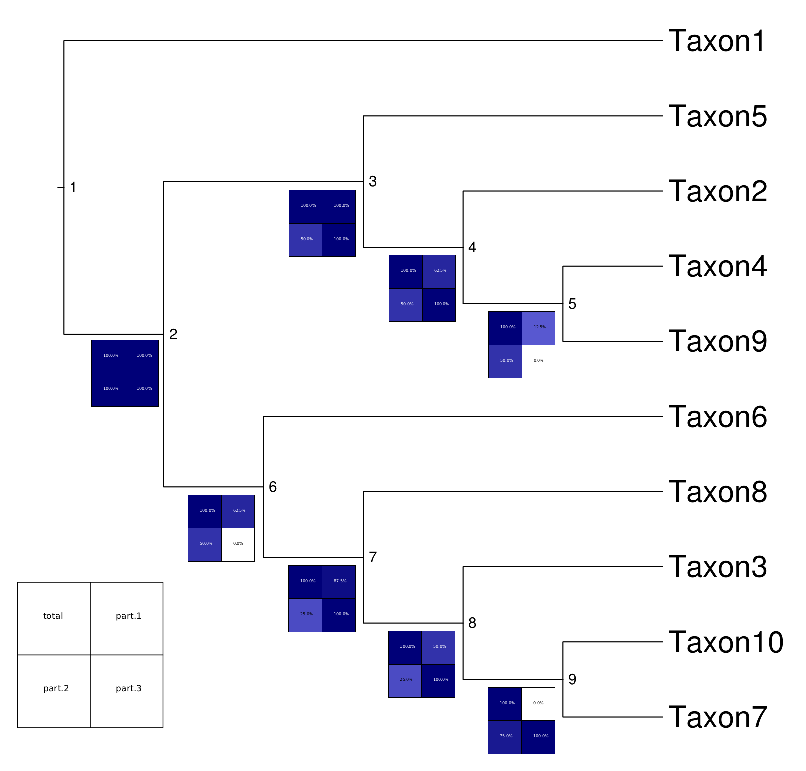
\includegraphics[scale=0.9]{figures/tut10/sens_plot.eps}}
	{\caption[Diagrama de sensibilidade (\textit{Navajo's rug})]{Diagrama de sensibilidade (\textit{Navajo's rug}) indicando como cada clado da análise simultânea se comporta nas análises individuais de cada partição. Quadrados em azul indicam a presença do clado de acordo com o mapa do \textit{plot} de sensibilidade ao lado do cladograma.}\label{tut10:fig:sens_plot}}
  \end{figure}

%%%%%%%%%%%%%%%%%%%%%%%%%%% FIM DA FIGURA TAP %%%%%%%%%%%%%%%%%%%%%

No exemplo abaixo iremos explorar o uso de YBYRÁ e FigTree para avaliar o resultado da análise de sensibilidade que foi executada na Seção \ref{tut10:sa:implementation}.

\subsubsection{YBYRÁ}\label{tut10:sa:evaluation:ybyra}

Toda documentação do YBYRÁ está diposponível do \href{https://gitlab.com/MachadoDJ/ybyra}{GitLab} do desenvolvedor. Para o propósito deste tutorial iremos apenas explorar como o YBYRÁ \footnote{Antes de iniciar este componente do tutorial execute o \textit{script} install\_dependencies.sh. Isso garantirá que você possui os programas necessários para executar os exercícios} pode ser utilizado para executar uma análise de sensibilidade.

O programa recebe instruções de um arquivo de configuração. No caso do exemplo que iremos apresentar aqui, essas instruções estão no arquivo \texttt{sensibilidade.conf}. Abra esse arquivo no \texttt{gedit}\footnote{Verifique se a numeração de linhas está habilidada no \texttt{gedit}. Se não estiver, vá em \textbf{Preferences} e clique em \textbf{Display line numbers}.} para que você siga as linhas que foram modificadas para que o YBYRÁ execute a análise de sensibilidade. As modificações feitas neste arquivo foram as seguintes:

\begin {myindentpar}{0.3cm}
\begin{enumerate}[\itshape i.]
	\item{Na linha 75 foi definida a \texttt{id} da análise (\textit{i.e.}, \texttt{sa\_aula}). A definição deste parâmetro no arquivo de configuração regula os nomes dos arquivos de \textit{output} (veja abaixo).}
	\item{Nas linhas 94--98 foram definidas as topologias que serão examinadas pelo programa em seus respectivos arquivos  (\textit{i.e.}, \texttt{trees\_m111.tre}, \texttt{trees\_m211.tre} e \texttt{trees\_m411.tre}). Em frente de cada arquivo, entre colchetes estão os \textit{labels} que serão utilizados nos diagramas de sensibilidade.}
	\item{Na linha 123 foi definida a topologia de referência, no caso aquela contida no primeiro arquivo da lista apresentada nas linhas 94--98. Entre colchetes está o nome do arquivo -- que é opicional. Por \textit{defaul}, YBYRÁ irá sempre utilizar a primeira topologia do primeiro arquivo da lista.}
	\item{Na linha 174 está definida o tipo de análise que você quer fazer -- nesse caso iremos comparar uma única topologia com as demais (1). Verifique as opções disponíveis no programa.}
	\item{Na linha 188 está definido que o YBYRÁ irá comparar clados -- opção 1 --, e não vértices de um diagrama não enraizados (\textit{i.e., splits}).}
	\item{Na linha 211 foi definido que você quer que o YBYRÁ imprima os diagramas de sensibilidade no formato SVG (\textit{Scalable Vector Graphics}) o que pode ser útil para gerar figuras como a apresentada acima (Figura \ref{tut10:fig:sens_plot}). A cor desses diagramas é especificada na linha 237.}
	\item{Uma vez configurado, basta executar o YBYRÁ com a seguinte linha de comando:}

	\shellcmd{ybyra\_sa.py -f sensibilidade.conf}\footnote{ esta linha de comando assume que você possui o programa instalado no seu sistema. A execução local deste programa pode ser feita da seguinte forma: ``\texttt{\$ python ybyra\_sa.py -f arquivo.conf}''. No diretório deste tutorial há uma versão simplificada deste arquivo de configuração chamado \texttt{sensibilidade\_simple.conf}.}

\end{enumerate}
\end{myindentpar}	

A execução do YBYRÁ gera uma série de arquivos de saída e o você deve consular o tutorial apresentado pelo desenvolvedor do programa, bem como a documentação do YBYRÁ, caso tenha interesse de saber o conteúdo específico de cada um deles. Para o propósito deste tutorial iremos descrever apenas alguns.

Após a execução diretório \texttt{tutorial\_10/} deverá conter os resultados da execução do YBYRÁ usando o arquivo de configuração \texttt{sensibilidade.conf}. Dentre estes arquivos, \texttt{LABELED\_sa\_aula.tre} contém a topologia de referência (\textit{i.e.}, \texttt{trees\_m111.tre}) com os nós anotados em referência aos arquivos \texttt{RUG\_000*\_sa\_aula.svg}. Estes últimos são arquivos vetoriais que mapeiam a frequência de cada clado presente na topologia de referência que foi encontrado nas demais topologias de acordo com o mapeamento apresentado no arquivo \texttt{RUG\_map\_sa\_aula.svg}. 

\subsubsection{FigTree \& Inkscape}\label{tut10:sa:evaluation:graphic}

O resultado da análise de sensibilidade executada acima está ilustrado na Figura \ref{tut10:fig:sensitivity}. Esta figura foi gerada utilizando dois aplicativos disponíveis na imagem do curso \href{http://tree.bio.ed.ac.uk/software/figtree/}{FigTree} e \href{http://www.inkscape.org/en/download/}{Inkscape}. Ambos programas podem ser executados em todas as plataformas (\textit{i.e.}, OS X, Linux e Windows) e são \textit{freeware}. Há dois vídeos em \texttt{tutorial\_10/videos/} que dão uma expliação geral de como usar o FigTree e o Inkscape nesse tutorial. O vídeo \texttt{figtree\_1.mp4} explica como o FigTree foi usado para gerar uma figura no formato SVG que representa a topologia que YBYRÁ utilizou para referenciar os diagramas de sensibilidade.  O vídeo \texttt{inkscape\_1.mp4} explica como o Inkscape foi utilizado para compor a Figura \ref{tut10:fig:sensitivity}. Se você já está familiarizado com esses aplicativos siga o tutorial a diante. No entanto, se você não os conhece é necessário que você assista esses vídeos antes de executar o exercício a seguir.

 %%%%%%%%%%%%%%%%%%%%%%%%%%% FIGURA TAP%%%%%%%%%%%%%%%%%%%%%%%%%%%
%  \vspace{-1em}
  \begin{figure}[H]
    %\ffigbox[\FBwidth]
       \centering
      {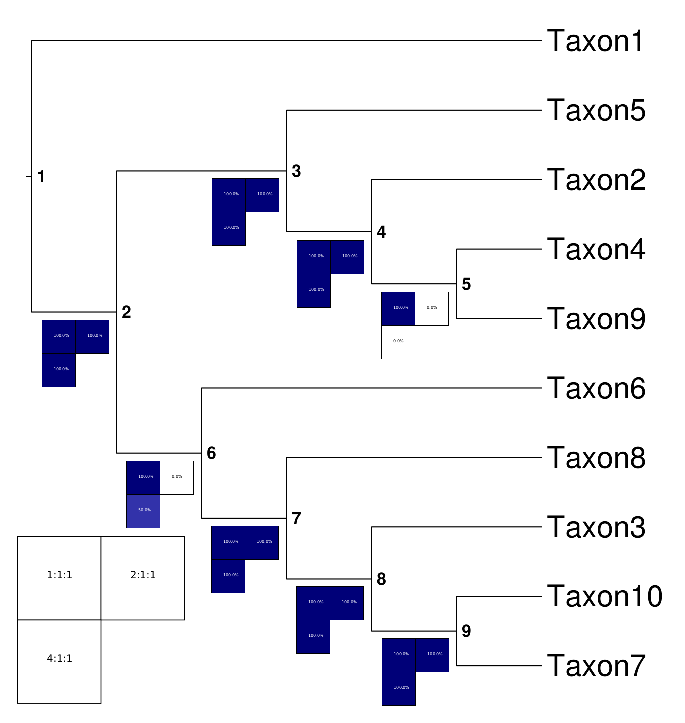
\includegraphics[scale=0.9]{figures/tut10/sensibilidade.eps}}
	{\caption[Diagrama de sensibilidade (\textit{Navajo's rug}) para parâmetros de alinhamento.]{Diagrama de sensibilidade (\textit{Navajo's rug}) para parâmetros de alinhamento indicando como cada clado da análise se comporta com relação aos custos diferenciais atribuídos para \textit{gaps}. Quadrados em azul indicam a presença do clado de acordo com o mapa do \textit{plot} de sensibilidade ao lado do cladograma.}\label{tut10:fig:sensitivity}}
  \end{figure}

%%%%%%%%%%%%%%%%%%%%%%%%%%% FIM DA FIGURA TAP %%%%%%%%%%%%%%%%%%%%%

\stepcounter{ex}
\begin{blackBlock}{\textbf{Exercicio 10.\arabic{ex}}}\label{tut10:ex:10.1}
Neste exercício você deverá fazer uma análise de sensibilidade considerando os dados em \texttt{partition1.fas}, \texttt{partition2.fas} e \texttt{partition3.tnt} aplicando os conceitos e componentes técnicos apresentados acima. Sua análise de sensibilidade deverá contemplar todas as matrizes de custos disponíveis no diretório associado a esse tutorial (\textit{i.e.}, \texttt{m111}, \texttt{m112}, \texttt{m121}, etc.).

\end{blackBlock}

\section{Comprimento de ramos \& Alinamentos implícitos}\label{tut10:sa:brlenia}

\subsection{Comprimento de ramos}\label{tut10:sa:brlen}

A versão atual de POY permite imprimir topologias com seus respectivos comprimentos de ramo. Este componente do programa era há muito esperado por seus usuários, pois comprimentos de ramos indicam o número aproximado transformações em determinado ramo e é um bom indicativo de divergência entre linhagens. Em POY, as topologias com comprimentos de ramos são requisitadas pelo comando \texttt{report(trees:(branches))}. Por \textit{default}, o comprimento de ramos é calculado por um único assinalamento de estado de caráter para cada determinado ancestral hipotético (\textit{i.e.}, HTU). No entanto, é possível solicitar ao POY que obtenha e reporte o número mínimo e máximo dos comprimentos de ramos com os comandos \texttt{report(trees:(branches:min))} e \texttt{report(trees:(branches:max))}, respectivamente.\\

\stepcounter{ex}
\begin{blackBlock}{\textbf{Exercicio 10.\arabic{ex}}}\label{tut10:ex:10.2}

Neste exercício você deverá fazer uma análise dos dados em \texttt{partition2.fas} em que todas as formas de cálculo de comprimento de ramos é registrada em arquivos de saída individuais. Posteriormente, avalie seus resultados e responda: Todos os ramos apresentam o mesmo comprimento? Justifique.

\end{blackBlock}

\begin{center}
\line(1,0){400}\\
\line(1,0){400}\\
\line(1,0){400}\\
\end{center}

\vspace{30pt}

\stepcounter{ex}
\begin{blackBlock}{\textbf{Exercicio 10.\arabic{ex}}}\label{tut10:ex:10.3}

Neste exercício você deverá fazer uma análise simultânea dos dados em \texttt{partition1.fas}, \texttt{partition2.fas} e \texttt{partition3.tnt} no qual o arquivo de saída é uma topologia contendo os comprimentos de ramos. Após a análise, você deverá gerar uma figura em FigTree.

\end{blackBlock}

\subsection{Alinhamento implícito}\label{tut10:sa:ia}

A otimização de alinhamentos em determinada topologia, definido no Tutorial \ref{tut9} como \textit{Tree Alignment Problem} \parencite[\textbf{TAP}; ][]{Sankoff_1975}, é o objetivo de POY. Como vocês observaram nos exercícios anteriores, é possível derivar um padrão filogenético a partir de sequências não-alinhadas por otimização direta na qual nenhuma referência ao alinhamento múltiplo é feito. \textcite{Wheeler_2003a} definiu como \textbf{alinhamento implícito} o procedimento no qual POY produz a diagnose de uma topologia baseada em sequências não alinhadas cujo resultado foi definido como ``\textit{'lines of correspondence' [that] link ancestor–descendent states and, when displayed as linearly arrayed columns without hypothetical ancestors, are largely indistinguishable from standard multiple alignment.}'' Embora o autor considere que em alguns caso a distinção seja difícil, alinhamentos implícitos são baseados em esquemas de sinapomorfias e em alguns casos, estes alinhamentos são visualmente estranhos, principalmente quando envolvem eventos de inserções e deleções \parencite[consulte][]{Wheeler_2003a}. 

O comando para que POY imprima o alinhamento implícito de uma ou mais topologias é \texttt{report(implied\_alignment)} ou sua versão abreviada \texttt{report(ia)}. No entanto, esse comando insere algumas linhas no início do arquivo que não permitem seu uso imediato por outros programas, como por exemplo BioEdit. Alternativamente, o comando \texttt{report(fasta)} produz a alinhamento implícito no formato FASTA, o que poderá ser utilizado imediatamente por outros programas que lêem esse formato de arquivo.\\

\stepcounter{ex}
\begin{blackBlock}{\textbf{Exercicio 10.\arabic{ex}}}\label{tut10:ex:10.3}

Você deverá gerar um alinhamento implícito resultante de uma análise filogenética por otimização direta em POY do arquivo \texttt{partition2.fas}. Após gerar esse alinhamento implícito, inspecione-o em BioEdit. Posteriormente, transforme esse alinhamento em uma matriz que possa ser analisada em TNT, faça uma busca e compile seus resultados no espaço abaixo.

\end{blackBlock}

\vspace{200pt}

\begin{center}
\line(1,0){400}\\
\line(1,0){400}\\
\line(1,0){400}\\
\end{center}




%%%%%%%%%%%%%%%%%%%%%%%%%%%% HERE ENDS TEXT AND ADDS REFERENCES %%%%%%%%%%%%%%%%%%%%%%%%%%%% 
\section{Referências}\label{tut10:refs}
\printbibliography[heading=none]
\end{refsection}
%  
